%\documentclass[handout]{beamer}
\documentclass{beamer}

\mode<presentation>
{
\usetheme{default}
\usefonttheme[onlymath]{serif}
%\usetheme{Singapore}
%\usetheme{Warsaw}
%\usetheme{Malmoe}
% \useinnertheme{circles}
% \useoutertheme{infolines}
% \useinnertheme{rounded}

\setbeamercovered{transparent=5}
}

\usepackage[english]{babel}
\usepackage[latin1]{inputenc}
\usepackage{textpos,alltt,listings,multirow,ulem,siunitx}
\newcommand\hmmax{0}
\newcommand\bmmax{0}
\usepackage{bm}

% font definitions, try \usepackage{ae} instead of the following
% three lines if you don't like this look
\usepackage{mathptmx}
\usepackage[scaled=.90]{helvet}
%\usepackage{courier}
\usepackage[T1]{fontenc}
\usepackage{tikz}
\usetikzlibrary[shapes,shapes.arrows,arrows,shapes.misc,fit,positioning]

% \usepackage{pgfpages}
% \pgfpagesuselayout{4 on 1}[a4paper,landscape,border shrink=5mm]

\usepackage{slashbox,multirow,listings,booktabs}
\usepackage{xspace}
\makeatletter
\DeclareRobustCommand\onedot{\futurelet\@let@token\@onedot}
\def\@onedot{\ifx\@let@token.\else.\null\fi\xspace}
\def\eg{{e.g}\onedot} \def\Eg{{E.g}\onedot}
\def\ie{{i.e}\onedot} \def\Ie{{I.e}\onedot}
\def\cf{{c.f}\onedot} \def\Cf{{C.f}\onedot}
\def\etc{{etc}\onedot}
\def\vs{{vs}\onedot}
\def\wrt{w.r.t\onedot}
\def\dof{d.o.f\onedot}
\def\etal{{et al}\onedot}
\makeatother

\usepackage{tikz}
\usetikzlibrary[shapes,shapes.arrows,arrows,shapes.misc,fit,positioning]

\usepackage{siunitx}
\DeclareSIUnit\year{a}
\DeclareSIUnit\byte{B}
\sisetup{retain-unity-mantissa = false}

\usepackage{fancyvrb}
\usepackage{minted}
\newminted{c}{gobble=2}
\newminted{python}{gobble=2}
%\newmint[cverb]{c}{} 
\newcommand\cverb[1][]{\SaveVerb[%
    aftersave={\textnormal{\UseVerb[#1]{vsave}}}]{vsave}}
\newcommand\cfunc[1][]{\SaveVerb[%
    aftersave={\textnormal{\UseVerb[#1]{vsave}\texttt{()}}}]{vsave}}
\newcommand\pyverb[1][]{\SaveVerb[%
    aftersave={\textnormal{\UseVerb[#1]{vsave}}}]{vsave}}
\def\asm#1{{\tt #1}}
\def\code#1{{\tt #1}}
\def\shell#1{{\tt \$ #1}}

\newcommand\email[1]{{\href{mailto:#1}{\nolinkurl{#1}}}}

\newcommand{\II}{\mathcal{I}}
\newcommand{\C}{\mathbb{C}}
\newcommand{\D}{\mathcal{D}}
\newcommand{\EE}{\mathcal{E}}
\newcommand{\F}{\mathcal{F}}
\newcommand{\I}{\mathcal{I}}
\newcommand{\N}{\mathcal{N}}
\newcommand{\PP}{\mathcal{P}}
\newcommand\Ppc{\ensuremath{\mathsf P}}
\newcommand{\bigO}{\ensuremath{\mathcal{O}}}
\newcommand{\R}{\mathbb{R}}
\newcommand{\Rz}{\mathcal{R}}
\newcommand{\QQ}{\mathcal Q}
\newcommand{\VV}{\mathcal V}
\newcommand{\ASM}{\mathrm{ASM}}
\newcommand{\RASM}{\mathrm{RASM}}

\newcommand{\kb}{\tt}
\newcommand{\Pk}[1]{\ensuremath{P_{#1}}}
\newcommand{\Qk}[1]{\ensuremath{Q_{#1}}}
\newcommand{\Pkdisc}[1]{\ensuremath{P_{#1}^{\text{disc}}}}
\newcommand{\Qkdisc}[1]{\ensuremath{Q_{#1}^{\text{disc}}}}
\newcommand{\blue}{\textcolor{blue}}
\newcommand{\green}{\textcolor{green!70!black}}
\newcommand{\red}{\textcolor{red}}
\newcommand{\brown}{\textcolor{brown}}
\newcommand{\cyan}{\textcolor{cyan}}
\newcommand{\magenta}{\textcolor{magenta}}
\newcommand{\yellow}{\textcolor{yellow}}
\newcommand{\mini}{\mathop{\rm minimize}}
\newcommand{\st}{\mbox{subject to }}
\newcommand{\lap}{\Delta}
\newcommand{\grad}{\nabla}
\newcommand\mtab{\hspace{\stretch{1}}}
\newcommand\ud{\,\mathrm{d}}
\newcommand\bslash{{$\backslash$}}
\newcommand\half{{\frac 1 2}}
\newcommand{\abs}[1]{\left\lvert #1 \right\rvert}
\newcommand{\bigabs}[1]{\big\lvert #1 \big\rvert}
\newcommand{\norm}[1]{\left\lVert #1 \right\rVert}
\newcommand\oneitem[1]{\begin{itemize} \item #1 \end{itemize}}
\newcommand\pfrak{{\mathfrak p}}
\newcommand\nfrak{{\mathfrak n}}
\newcommand\ff{\bm f}
\newcommand\mm{\bm m}
\newcommand\nn{\bm n}
\newcommand\uu{\bm u}
\newcommand\vv{\bm v}
\newcommand\ww{\bm w}
\newcommand\DD{D}
\newcommand{\tcolon}{\!:\!}
\DeclareMathOperator{\sgn}{sgn}
\DeclareMathOperator{\card}{card}
\DeclareMathOperator{\trace}{tr}
\DeclareMathOperator{\erf}{erf}
\DeclareMathOperator{\sspan}{span}
\renewcommand{\bar}{\overline}
% \DeclareMathOperator{\divergence}{div}
% \renewcommand\div\divergence
\renewcommand{\div}{{\nabla \cdot}}
\newcommand\spliceop{\leftrightsquigarrow}
\newcommand\splice[5]{{#1} \overset{#5}{\underset{#3,#4}{\leftrightsquigarrow}} {#2}}
\newcommand{\ip}[2]{{\left\langle #1, #2 \right\rangle}}
\newcommand{\Linfty}{{L^\infty}}

% Dimensionless numbers
\newcommand{\Peclet}{{\mathrm{Pe}}}
\newcommand{\Reynolds}{{\mathrm{Re}}}
\newcommand{\Rayleigh}{{\mathrm{Ra}}}
\newcommand{\Mach}{{\mathrm{Ma}}}
\newcommand{\Prandtl}{{\mathrm{Pr}}}
\newcommand{\Grashof}{{\mathrm{Gr}}}

\newcommand{\PETSc}{{PETSc}}
\newcommand{\Dohp}{{Dohp}}
\newcommand\libmesh{\texttt{libMesh}}
\newcommand\dealii{\texttt{Deal.II}}
\newcommand\MatMult{\cverb|MatMult|}
\newcommand\MatSolve{\cverb|MatSolve|}
\newcommand{\secref}[1]{{Section~\ref{#1}}}
\newcommand{\chapref}[1]{{Chapter~\ref{#1}}}
\newcommand{\figref}[1]{{Figure~\ref{#1}}}
\newcommand{\tabref}[1]{{Table~\ref{#1}}}
\newcommand\AIJ{{\cverb|AIJ|}}
\newcommand\AIJInode{\cverb|AIJ|/\cverb|Inode|}
\newcommand\BAIJ[1][]{\ifthenelse{\equal{#1}{}}{\cverb|BAIJ|}{\ensuremath{\cverb|BAIJ|(#1)}}}
\newcommand\SBAIJ[1][]{\ifthenelse{\equal{#1}{}}{\cverb|SBAIJ|}{\ensuremath{\cverb|SBAIJ|(#1)}}}
\newcommand\todo[1]{{\color{red}\bf [TODO: #1]}}
\newcommand\tf[1]{\hat{#1}}     % test functions


\title{Towards Interactive Analysis of Regional Ice Flow}

\author{Iulian Grindeanu, Jed Brown, Dmitry Karpeev, Barry Smith, Tim Tautges, Jean Utke}


% - Use the \inst command only if there are several affiliations.
% - Keep it simple, no one is interested in your street address.
\institute[ANL]
{
  Argonne National Laboratory
}

\date{2011-06-22}

% This is only inserted into the PDF information catalog. Can be left
% out.
\subject{Talks}


% If you have a file called "university-logo-filename.xxx", where xxx
% is a graphic format that can be processed by latex or pdflatex,
% resp., then you can add a logo as follows:

% \pgfdeclareimage[height=0.5cm]{university-logo}{university-logo-filename}
% \logo{\pgfuseimage{university-logo}}



% Delete this, if you do not want the table of contents to pop up at
% the beginning of each subsection:
% \AtBeginSubsection[]
% {
% \begin{frame}<beamer>
% \frametitle{Outline}
% \tableofcontents[currentsection,currentsubsection]
% \end{frame}
% }

% If you wish to uncover everything in a step-wise fashion, uncomment
% the following command:

%\beamerdefaultoverlayspecification{<+->}

\begin{document}
\lstset{language=C}
\normalem

\begin{frame}
\titlepage
\end{frame}

\newcommand\smallterm[1]{{\color{gray} #1}}
\begin{frame}{Conservative two-phase formulation}
  Find momentum density $\rho\uu$, pressure $p$, and total energy density $E$:
  \begin{gather*}
    (\rho\uu)_t + \div (\smallterm{\rho\uu\otimes\uu} - \eta D\uu_i + p\bm 1) - \rho \bm g = 0 \\
    \rho_t + \div \rho\uu = 0 \\
    E_t + \div \big((E+p)\uu - k_T\nabla T - k_\omega\nabla\omega \big) - \eta D\uu_i\tcolon D\uu_i - \smallterm{\rho\uu\cdot\bm g} = 0
  \end{gather*}
\begin{itemize}
\item Solve for density $\rho$, ice velocity $\uu_i$, temperature $T$, and melt fraction $\omega$ using constitutive relations.
  \begin{itemize}
  \item Simplified constitutive relations can be solved explicitly.
  \item Temperature, moisture, and strain-rate dependent rheology $\eta$.
  \item High order FEM, typically $Q_3$ momentum \& energy, SUPG (yuck).
  \end{itemize}
\item DAEs solved implicitly after semidiscretizing in space.
\item Newton solver converges quadratically.
\item Thermocoupled steady state in one nonlinear solve
  \begin{itemize}
  \item no time stepping needed, total cost similar to 3 semi-implicit steps
  \item useful for inverse problems and stability analysis
  \end{itemize}
\item (Somewhat) robust preconditioning using nested field-split
\end{itemize}
\end{frame}

\begin{frame}{Block on inclined plate, nominal $\Reynolds = 0.24$, $\Peclet = 120$}
  \begin{columns}
    \begin{column}{0.5\textwidth}
      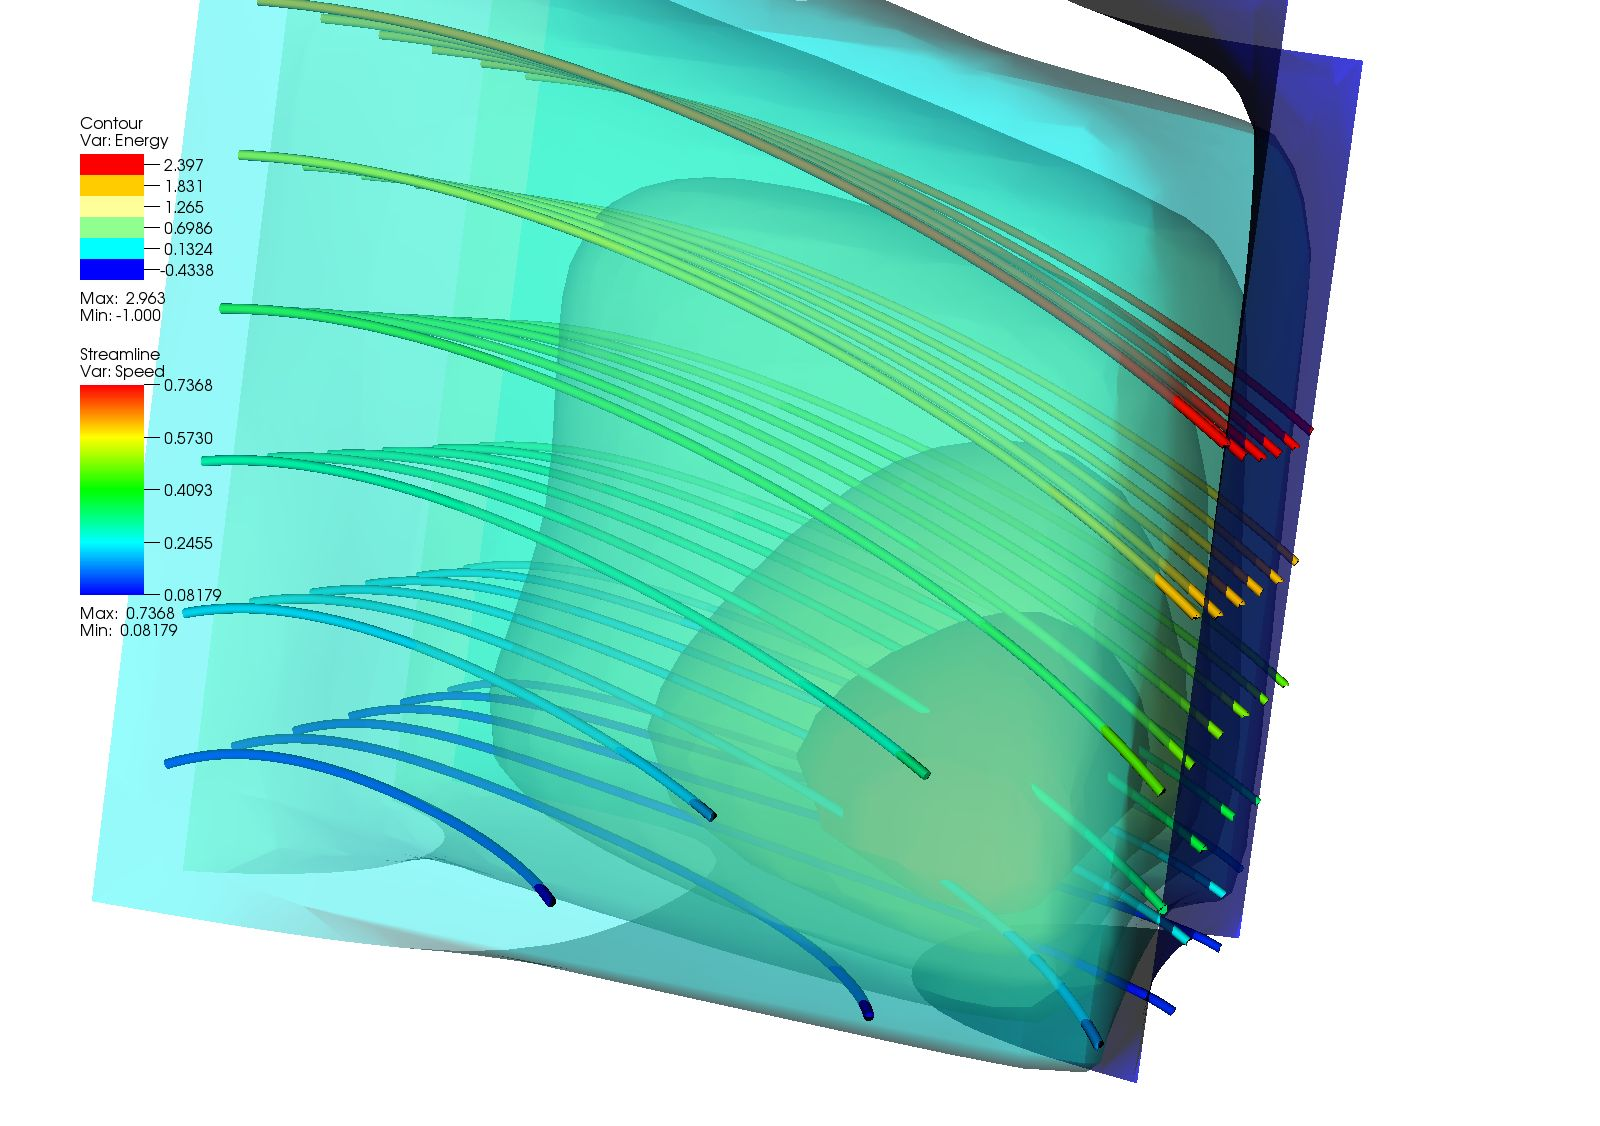
\includegraphics[width=1.3\textwidth]{figures/VHTNondimEnergy} \\
      Contours of Energy, melt fraction up to 15\%, density ratio 2.
    \end{column}
    \begin{column}{0.5\textwidth}
      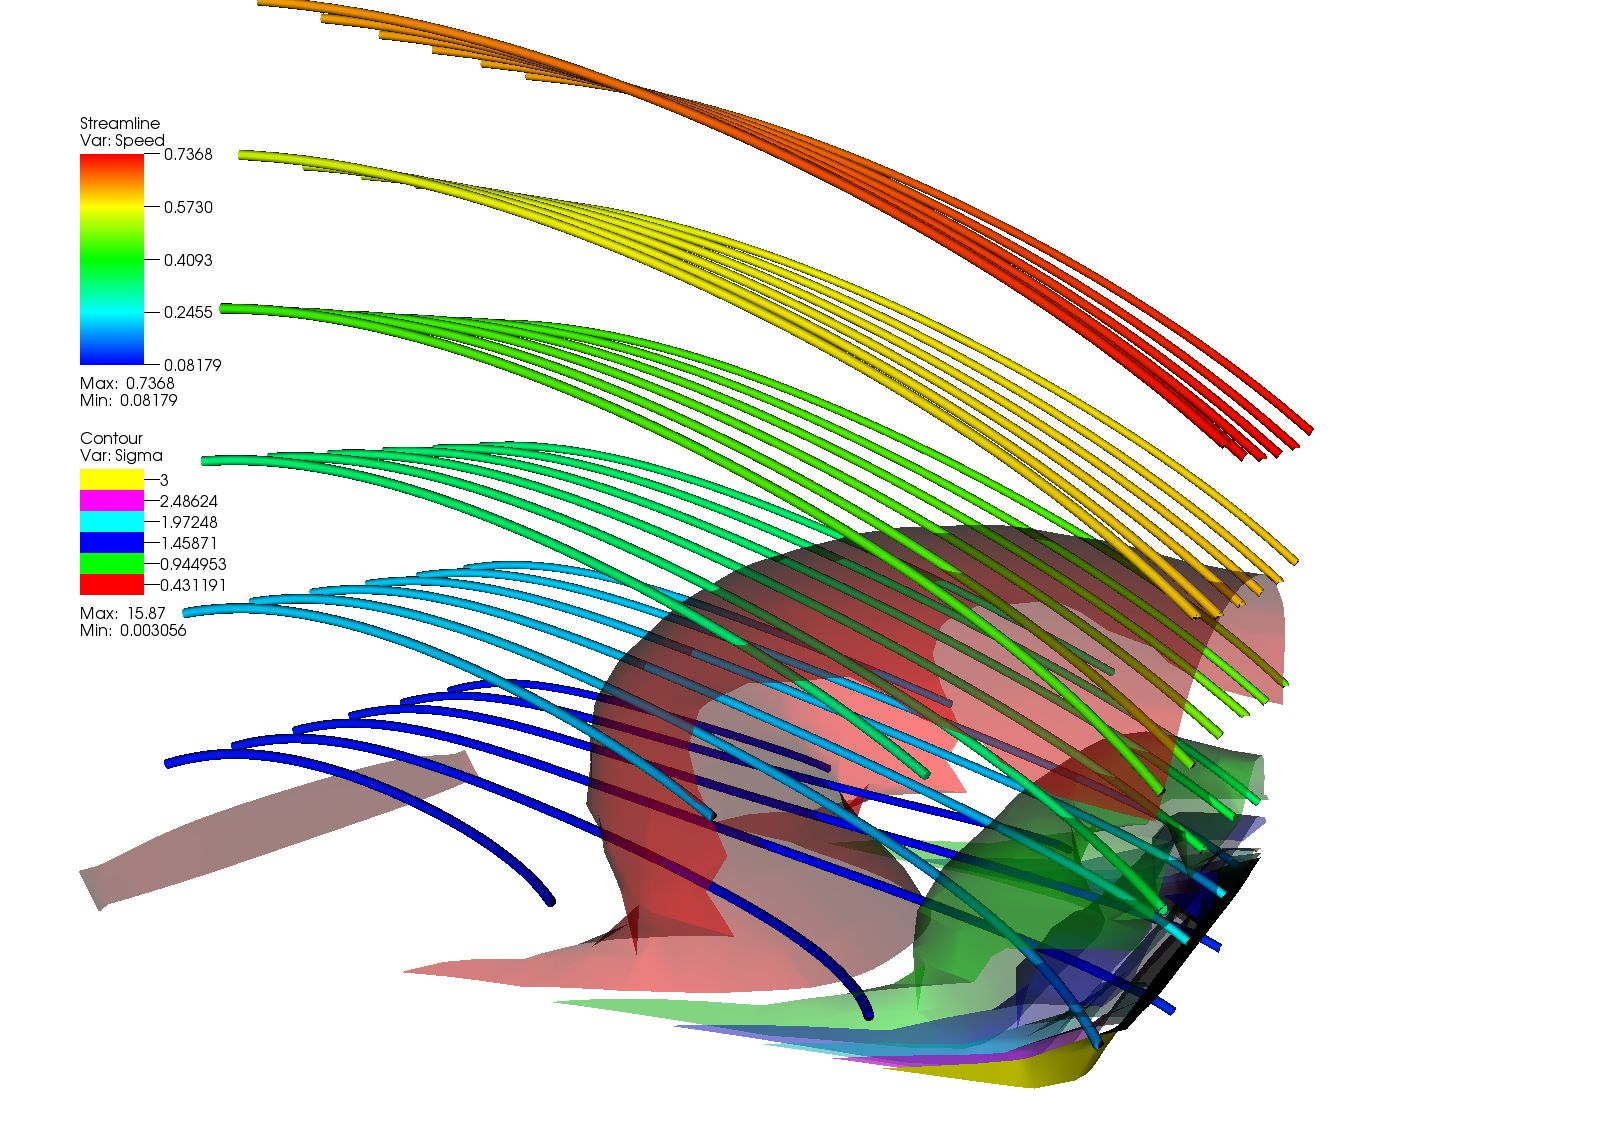
\includegraphics[width=1.3\textwidth]{figures/VHTNondimSigma} \\
      Contours of viscous heat production, $1/r$ singularity at corners.
    \end{column}
  \end{columns}
\end{frame}

\begin{frame}[shrink=5]{Performance of assembled versus unassembled}
  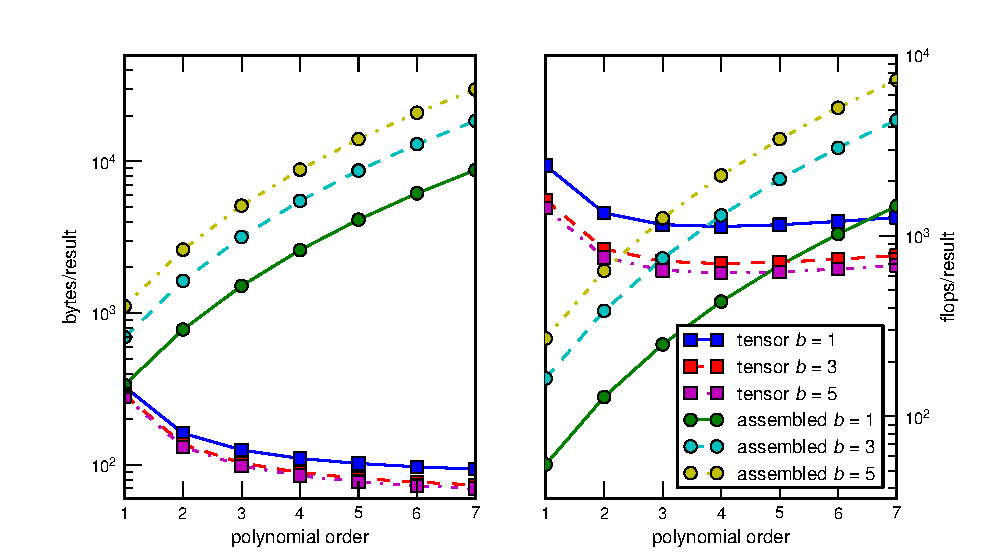
\includegraphics[width=\textwidth]{figures/TensorVsAssembly} \\
  \begin{itemize}
  \item High order Jacobian stored unassembled using coefficients at quadrature points, can use local AD
  \item Choose approximation order at run-time, independent for each field
  \item Precondition high order using assembled lowest order method
  \item Implementation $> 70\%$ of FPU peak, SpMV bandwidth wall $< 4\%$
  \end{itemize}
\end{frame}


\end{document}
